%Basics
\documentclass[aps, prl, reprint, a4paper, english, 12pt, twocolumn]{revtex4}
\bibliographystyle{apsrev4-1}
\usepackage[utf8]{inputenc}
\usepackage{babel}

%Symbols and scientifics
\usepackage{amsmath}
\usepackage{commath}
\usepackage{amsfonts}
\usepackage{amssymb}
\usepackage{physics}
\usepackage{mathtools}
\usepackage{siunitx}
\sisetup{
per-mode = fraction ,
round-mode = figures ,
round-precision = 3 ,
scientific-notation = engineering ,
output-decimal-marker = {.} ,
exponent-product = \times ,
separate-uncertainty = true ,
uncertainty-separator = \ ,
output-product = \cdot ,
quotient-mode = fraction ,
range-phrase = - ,
range-units =  single ,
inter-unit-product = \ensuremath{{\cdot{}}} ,
number-unit-product = \ ,
multi-part-units = single ,
}
\usepackage{units}

%Appendix, TOC and Bibliography
\usepackage{appendix}
\renewcommand\appendixtocname{Appendices}
%\usepackage[nottoc]{tocbibind}
\usepackage[lastpage,user]{zref}

%Figures
\usepackage[svgnames]{xcolor} % Required to specify font color
\usepackage{tikz}
\usetikzlibrary{shadings}
\usepackage{float}
\usepackage{rotating}
\usepackage{graphicx}
\usepackage{wrapfig}
\usepackage[rmargin=2.5cm, tmargin=2.5cm, lmargin=2.5cm, bmargin=2.5cm]{geometry}
\usepackage{xcolor}
\usepackage{etoolbox}
\usepackage{verbatim}
\usepackage[space]{grffile}
\usepackage[final]{pdfpages}
\usepackage{array}
\usepackage{multirow}

%Header footer
\usepackage{fancyhdr}
\pagestyle{fancy}
\lhead{F. G. Kristensen,\\C. V. Sørensen og R. K. F. Wiuff}
\chead{Nanomechanics for graphene membranes\\}
\rhead{10/1-2018\\Course 34029: Physics Project}
\cfoot{Side \thepage\, af \zpageref{LastPage}}
\renewcommand{\headrulewidth}{0.4pt}
\renewcommand{\footrulewidth}{0.4pt}

%Text tools
\usepackage[normalem]{ulem}
\usepackage{import}
\usepackage{newclude}
\usepackage{url}
\usepackage{lipsum}
\usepackage{microtype}
\usepackage{hyperref}
\hypersetup{
  colorlinks   = true, %Colours links instead of ugly boxes
  urlcolor     = blue, %Colour for external hyperlinks
  linkcolor    = blue, %Colour of internal links
  citecolor   = red %Colour of citations
}
\usepackage[capitalise]{cleveref}
\usepackage{enumitem}
\usepackage{booktabs}
\usepackage{silence}
\WarningFilter{revtex4-1}{Repair the float}

%Python
\usepackage{minted}
\usemintedstyle{monokai}
\renewcommand{\listoflistingscaption}{Listings}

%Definitions and new commands
\setlength{\parindent}{0pt}
\setlength{\parskip}{1ex plus 0.5ex minus 0.2ex}
\newcommand{\logas}[1]{\log_{_{10}}{\left( #1 \right)}}
\newcommand{\sins}[1]{\sin{\left( #1 \right)}}
\newcommand{\tans}[1]{\tan{\left( #1 \right)}}
\newcommand{\coss}[1]{\cos{\left( #1 \right)}}
\newcommand{\sinas}[1]{\sin{\left( #1 \degr \right)}}
\newcommand{\tanas}[1]{\tan{\left( #1 \degr\right)}}
\newcommand{\cosas}[1]{\cos{\left( #1 \degr\right)}}
\newcommand{\lnas}[1]{\mathrm{ln}\left( #1 \right)}
\newcommand{\degr}{^{\circ}}
\newcommand{\me}{\mathrm{e}}
\newcommand{\eula}[1]{ \dpd{L }{#1} - \dod{}{t}\left(\dpd{L}{\dot{#1}}\right)}
\begin{document}

%Titlepage herunder:
\begin{abstract}
 \begin{description}
  In this report we will focus on nanomembranes and analyse how this react when a force is applied to them. Nanomembranes can be fabricated via the method of chemical vapor deposition (CVD) and this have been test in the lab by using electrostatic gates \cite{Zande2010}. There are also examples of using lasers to drive a vibration in a membrane \cite{Davidovikj2016} but both of this membranes however are way lager then the ones we will be studying in this report. the concept of carbon nanomembranes have existed for a couple of years all ready so what we are going to focus on are the the smallest nanomembranes that can be made right now.
 \end{description}
\end{abstract}

\title{Nanomechanics for graphene membranes}
\date{10/1-2018}
\author{Frederik Grunnet Kristensen (s164003)}
\email[E-mail at ]{s164003@student.dtu.dk}
\author{Christoffer Vendelbo Sørensen (s163965)}
\email[E-mail at ]{s163965@student.dtu.dk}
\author{Rasmus Kronborg Finnemann Wiuff (s163977)}
\email[E-mail at ]{s163977@student.dtu.dk}
\affiliation{Technical University of Denmark}
\homepage[Homepage of the Technical University of Denmark ]{http://www.dtu.dk/english/}

\maketitle

\pagenumbering{arabic}

\tableofcontents
\thispagestyle{empty}
\newpage
\setcounter{page}{1}

%Text
\section{Introducing the project}
% !TEX root = ../Main.tex

Since the isolation and characterisation of
Graphene in 2004 by Andre Geim and
Konstantin Novoselov, scientists have marvelled over the physical properties and potential
application of Graphene. Being a relatively new material, many aspects and ideas are being
investigated and researched at all times. Graphene yield extreme tensile strength as well as
extreme electric conductivity, yet its structure is fairly simple. Graphene consists solely of
carbon atoms thus making it easy to simulate using specialised software, since carbon atoms are greatly understood in terms of chemical
bonding.
As graphene is a very versatile material the possibilities for research in simulation enviroments are virtually limitless.
Therefore it is basically possible to make experiments limited only by imagination, in order
to discover new properties and possible applications of graphene. This saves resources
before entering the lab, where the simulated reality is tested.

In this rapport we will simulate and analyse the properties of nanomembranes as done in the papir "Visualizing the Motion of Graphene Nanodrums"\cite{Davidovikj2016}, which Figure \cref{Motivation} stems from. It shows how phonos travel through this membranes. However there this article,as many others, focuses on membranes in the micro-scale we will examine if this same phenomenons are found at the nano-scale. To do this we start by considering at ideal system of just one sheet of carbon atoms.
To make a more praticel membrane we will investigate if you can create the same membrane effects if you take a graphene layer and put it on top of a substrate with different sized and shaped holes, to form
form this nanomembrane and this is the that we will be looking at. It is expected possible to create such a nanomembrane at the
size of few tens of nanometers at Nanotech with Block-copolymer lithography or TEM
structuring of a substrate. In a virtual environment, it is possible to simulate phonons
in the graphene atop of these holes in the membrane. The purpose of this project is to
simulate phonons in the nanomembrane and find the optimal conditions for producing
phonons in the terahertz spectrum.
We will employ the software Atomistic ToolKit (ATK) to calculate phonon properties
of membranes as well as performing molecular dynamics of the excited membrane. The
software will enable prompt setup of relevant structures so that more time is free to analysis
and actual simulations.
\begin{figure}
    \centering
    \includegraphics[width=0.5\textwidth]{Figures/NanoDrums.png}
    \caption{Visualizing resonant motion. (a–h) Top, experimental data; bottom, finite-element calculation. The modes predicted by the calculation are indexed by (m,n). Panels b and c show that the nanodrum hosts a split degenerate (1,1) mode, while also the (2,1) mode is split, as is shown in panels d and e. The displacement profile measured in panel f resembles a (0,2) mode, which is distorted due to an imperfection as discussed in the main text. Panels g and h reveal a degenerate (1,2) mode. Scale bars: 1 $\mathrm{\mu m}$.\cite{Davidovikj2016}}
    \label{Motivation}
\end{figure}
\section{Introduciton to Lattice Geometry, Nanomechanics and Atomistix ToolKit}
% !TEX root = ../Main.tex

\subsection{Lattice Geometry}
In order to set up the simulation environment the basic geometry of system must be defined. Using generating vectors as well as unitcells the structure and holes of the graphene sheet will be defined within this geometry.
\subsubsection{Bravais Lattice \& Generating Vectors}\label{BLGV}
At first we want to specify a Bravais lattice for the graphene-layer. The Bravais lattice is a lattice that is invariant under translation which means that the lattice does not change when you translate it with the vector
\begin{equation}
 \mathbf{T}=n\mathbf{a_{1}}+m\mathbf{a_{2}}\ \ \ \mathbf{a_{1}},\mathbf{a_{2}} \in \mathbb{R}^{2}
\end{equation}
Where $n,m \in \mathbb{Z}$ and $\mathbf{a_{1}}$, $\mathbf{a_{2}}$ are the generating vectors for the space lattice. Moreover, all the points in the lattice are given by
\begin{equation}
 \mathbf{R}=(nd,md)
\end{equation}
where $d$ is the spacing between the lattice points and $n,m$ can be both positive and negative integers. \\
As we are working with graphene which is carbon atoms arranged in a hexagonal structure, we want to choose a hexagonal Bravais lattice and define our generating vectors accordingly. Both generating vectors start at the center of a hexagon. This gives the generating vectors $\mathbf{a_{1}}=(d,0)$ \& $\mathbf{a_{2}}=\left(-\dfrac{d}{2},\dfrac{\sqrt{3}d}{2}\right)$. In \cref{hexagon} a drawing of the lattice with its generating vectors is shown.\\
As the carbon-carbon bondlength in graphene is \SI{1.42}{\angstrom}, the distance between the lattice points  in the Bravais lattice is $d=\SI{2.4612}{\angstrom}$. This gives the numerical form of the analytical derived expression for the generating vectors  $\mathbf{a_{1}}$ \& $\mathbf{a_{2}}$. \\
$\mathbf{a_{1}}=(\SI{2.4612}{\angstrom},0)$ \& $\mathbf{a_{2}}=\left(-\SI{1.2306}{\angstrom},\SI{2.1315}{\angstrom}\right)$. \\These are the vectors that will be employed during simulation.
\begin{figure}
 \centering
 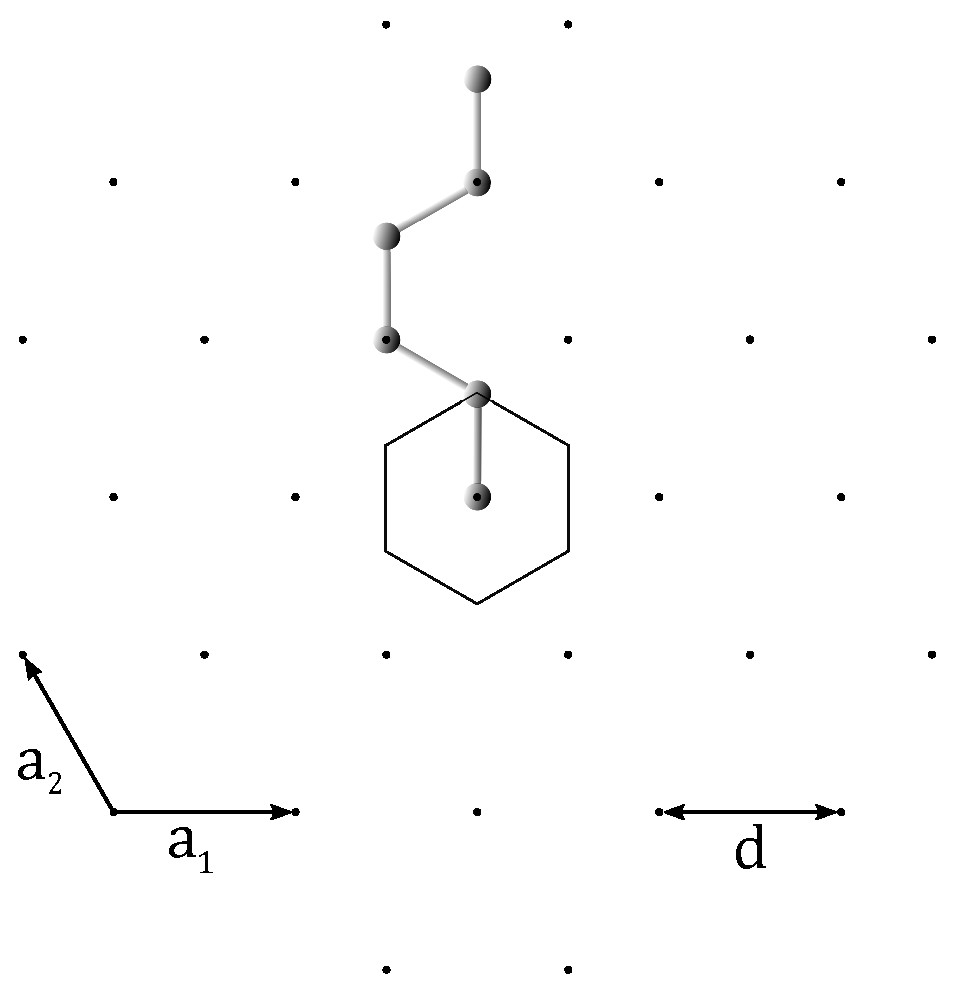
\includegraphics[width=0.5\textwidth]{Figures/hexagon2.eps}
 \caption{Hexagonal Bravais lattice structure with generating vectors $\mathbf{a_{1}}$ \& $\mathbf{a_{2}}$. The Hexagon in the middle with the solid lines is unit cell and the shaded elements are the carbon atoms placed in the lattice.}
 \label{hexagon}
\end{figure}

% !TEX root = ../Main.tex

\subsection{Nanomechanics}
This following section will focus on the mechanics of the know defined geometry of the Graphene sheet. It will incorporate boundary conditions in two dimensions, Hooke's law, the normal modes of the lattice as well as phonons. (relaxation energy)

\subsubsection{Boundary Conditions in Two Dimensions}
\todo[inline]{Write section}
 
\input{sections/MD.tex}
\subsection{Atomistix ToolKit: ATKPython and Nanolanguage}
The Python script creating the lattice and tags are printed and commented in the Appendix on \cpagerefrange{NSCstart}{NSCend}

%End of text

%Bibliography herunder:
\newpage

\bibliography{Physics-Project-Nanomechanics-for-Graphene-Membranes}

\newpage
\listoffigures
\listoftables
\listoflistings
\onecolumngrid
\newpage
%Appendicer herunder:
% !TEX root = Main.tex

\appendix
\appendixpage
\addappheadtotoc
%\section{Animation of \nth{9} mode}
%\begin{center}
%  \animategraphics[autoplay,loop,width=\textwidth]{60}{VNL/Frames/frame}{1}{60}
%\end{center}
%Section 1 herunder:

%Section 2 herunder:

\end{document}
